
Entriamo nell'attualità delle problematiche più recenti che riguardano la normativa del diritto d'autore a livello europeo e italiano, affrontando questioni che impattano anche sulle nostre esperienze quotidiane.  

\section{Attualità nazionale ed europea nel diritto d'autore}

Essenzialmente tre tematiche:
\begin{itemize}
    \item Regolamento AGCOM sul diritto d'autore (DdA): AGCOM ha iniziato in tempi non sospetti a prendere potere in ambiti relativi al diritto d'autore e ad agire in modo energico (solo ultimamente depotenziato)
    \item Gestione collettiva del DdA: SIAE e il monopolio della problematica 
    \item Riforma Europea del DdA e recepimento negli stati membri: riforma molto recente ad attuazione ancora più recente nell'ordinamento italiano

\end{itemize}

Le tematiche sono numerosissime e coinvolgono le opinioni personali dei cittadini più di quanto non facciano altri ambiti.

\subsection{Regolamento AGCOM 2014: tutela del DDA sulle piattaforme digitali}

AGCOM è da quasi dieci anni che si occupa di dirimere controversie che riguardano il diritto d'autore online, in particolare relativamente alla pirateria, da prima ancora che nascessero le piattaforme di streaming che consentono l'abbonamento ai servizi che ``rinunciano" alla pirateria sistematica (che faceva anche perdere tempo con le connessioni lente e i download di file enormi). 

A partire dal 2014 AGCOM ha deciso di agire nel panorama dei diritti dei creatori di contenuti condivisi illegalmente su varie piattaforme online. 

Tramite sito web dell'AGCOM è possibile segnalare violazioni di DdA: normalmente la segnalazione avviene da parte di case editrici/produttori che vengono a conoscenza della violazione dei diritti d'autore dei contenuti dei propri creatori. 

Il regolamento per la tutela del DdA sostanzialmente garantisce agli utenti la facoltà di segnalare delle violazioni (contenuti che appaiono in siti che non hanno l'autorizzazione a pubblicarli) e a questo punto l'AGCOM utilizza tutti i suoi poteri para-giurisdizionali (superando quindi tutte le limitazioni e ritardi in termini di tempo e denaro derivati dalla burocrazia ``tradizionale") per istituire una procedura molto breve che verifica la violazione, notificando il soggetto che viola il DdA e intimando la rimozione dei contenuti illeciti entro tre giorni (procedura di \textit{notice and takedown}). 
Nel momento in cui non avviene la rimozione spontanea dei contenuti si va verso l'oscuramento del sito. 

C'è la possibilità di ricorrere a citazione in giudizio ``tradizionale" ma l'azione dell'AGCOM ha una rapidità di esecuzione molto maggiore.

Il regolamento contiene una serie di punti controversi legati all'ambito di applicazione molto vasto (forse troppo): cosa è definibile come opera multimediale soggetta a questo regolamento?

\subsubsection{Il caso Telegram e piattaforme di messaggistica istantanea}

Il caso Telegram è sorto durante il periodo della pandemia in cui venivano condivisi i pdf di testate giornalistiche su gruppi o canali aventi migliaia di partecipanti. 

In questo caso AGCOM aveva poteri limitati legati al fatto che il suo regolamento riguardava Internet e non le piattaforme di messaggistica o i social network. 
AGCOM ampliò il proprio potere in modo da poter gestire violazioni del DdA anche in ambito di condivisione sui social e non solamente su siti web.

\subsection{Gestione collettiva del diritto d'autore}
La gestione collettiva del diritto d'autore in Italia avviene grazie alla SIAE, ossia un ente che si occupa di attuare la normativa sul diritto d'autore. Nella legge sul diritto d'autore è esplicitamente nominata la SIAE. 
Tramite sito web della SIAE è possibile acquisire il diritto di utilizzare per un determinato periodo di tempo un'opera di creatori protetti dal diritto d'autore. 

La cessione dei diritti, la ripartizione dei proventi, etc. sono aspetti afferenti al diritto privato. Peraltro, ciascun diritto attinente a un'opera ha una propria storia diversa dagli altri (es. diritto di copia ha un'origine diversa dal diritto di cessione). 

La SIAE nasce come soggetto pubblico di intermediazione e assume questo ruolo in modo esclusivo fino al marzo 2017.
Ruoli:
\begin{enumerate}
    \item Concessione di licenze e autorizzazioni per l'utilizzazione economica di opere tutelate
    \item Percezione dei proventi derivanti da dette licenze e autorizzazioni
    \item Ripartizione dei proventi medesimi tra gli aventi diritto
\end{enumerate}

Dal marzo 2017 il monopolio da parte della SIAE e l'eccessiva standardizzazione furono ridotti grazie all'introduzione di organismi alternativi per la gestione collettiva.

\subsubsection{Apertura del mercato della gestione collettiva}
Direttiva europea (c.d. Barnier) 2014/26/UE

I titolari del diritto d'autore possono affidare la tutela dei propri diritti alla società che preferiscono all'interno dell'UE. 

Questa direttiva definisce:
\begin{itemize}
    \item OGC: Gli organismi di gestione collettiva (autorizzati per legge o in base a una cessione di diritti, una licenza o accordo contrattuale) autorizzati a gestire i diritti d'autore o quelli ad essi connessi per conto di più di un titolare dei diritti, a vantaggio collettivo di tali titolari. Tali organismi sono detenuti o controllati dai propri membri e sono organizzati senza fini di lucro (in Italia la SIAE)
    \item EGI: entità di gestione indipendente. Si tratta di organismi autorizzati a gestire i DdA di più di un titolare dei diritti; tale organismo non è né detenuto né controllato dai titolari dei diritti ed è organizzato a fini di lucro (es. YouTube, Spotify, Soundreef)
\end{itemize}

In Italia il monopolio della SIAE è stato abolito dall'introduzione di LEA (senza scopo di lucro).

\subsection{La riforma europea del DDA e recepimento negli Stati membri}

Nel 2016 arriva una proposta direttiva del Parlamento Europeo e del Consiglio per rendere le norme UE sul diritto d'autore più adatte al mercato interno, adattare le norme sul DdA alle nuove tecnologie, migliorare l'accesso ai contenuti disponibili online, migliorare il funzionamento del mercato dei diritti d'autore, equilibrare i guadagni dei creatori delle opere e di chi invece le utilizza soltanto…

La direttiva nasce dalla volontà di adattare le regole attualmente vigenti negli Stati dell'UE a nuove forme di utilizzo delle opere protette.  In particolare vuole riequilibrare il disavanzo di valore subito dagli autori e altri titolari di diritti a fronte di una fruizione e di un utilizzo incontrollato delle proprie opere sul web (\textbf{value gap}).

4 settori di intervento:
\begin{itemize}
    \item Introduzione di alcune misure finalizzate ad adeguare le eccezioni al diritto d'autore per la riproduzione di opere (es. risolvere problemi legati alla diffusione non autorizzata di parti di opere su siti/piattaforme terzi)
    \item Istituzione di un meccanismo giuridico per facilitare gli accordi di licenza per opere fuori commercio
    \item Estensione dei diritti della direttiva 2001/29/CE (diritti esclusivi di riproduzione e comunicazione al pubblico) agli editori di giornale per l'utilizzo digitale delle loro pubblicazioni 
    \item Imposizione agli hosting providers dell'obbligo di retribuire i detentori di diritti
\end{itemize}

\subsubsection{Nuova direttiva copyright europea 2018: gli articoli più dibattuti}

\begin{itemize}
    \item Articolo 15 (ex Articolo 11) -- \textbf{link tax}
    
    Ogni stato membro deve assicurarsi che gli editori dei siti di notizie ricevano una consona ed equa remunerazione per l'uso dei loro materiali da parte dei fornitori di servizi nella società dell'informazione, cioè da parte delle piattaforme.

    Una volta le notizie riportate sui siti news erano più lunghe (titolo, fotografia, riassunto), mentre oggi si tende a vedere solo il titolo della notizia: si tratta di un metodo per aggirare la percentuale di opera condivisa oltre la quale bisognerebbe remunerare la testata giornalistica fonte della notizia.
    
    \textbf{Posizioni pro}: l'informazione di qualità costa e va pagata degli utenti e dai social network; molti utenti si limitano a titoli e brevi estratti sulle piattaforme e non visitano i siti delle testate giornalistiche per cui la pubblicità viene spesso piazzata sulla piattaforma e non sul sito della testata giornalistica (dove finisce per rendere molto meno al giornale). Chiaramente a favore della link tax c'erano gli editori che accusano i social network e motori di ricerca di usare i loro contenuti senza fornire in cambio remunerazione economica.
    
   \textbf{Posizioni contro}: far pagare le news favorisce la maggiore diffusione di fake news e notizie di bassa qualità (senza fact checking); se piattaforme che non sono grandi e non guadagnano troppo dalle pubblicità per veicolare informazione devono pagare gli editori delle notizie finiscono per perderci. Contro la link tax ci sono tutti gli organizzatori per la tutela della libertà su internet e le piattaforme che dicono di fare già gli interessi degli editori (secondo le piattaforme le visualizzazioni delle testate giornalistiche derivano già principalmente dalle notizie pubblicate sulle piattaforme stesse quindi esse non dovrebbero ritenersi in debito nei confronti degli editori)

   \item Articolo 17 (ex Articolo 13) -- fingerprinting
   
   Prevede che le piattaforme online esercitino una sorta di controllo attivo su ciò che viene caricato dai loro utenti, in modo da escludere a priori la pubblicazione di contenuti protetti dal copyright e sui quali non si detengono diritti. 

   Le piattaforme dovrebbero effettuare una sorta di filtraggio dei contenuti: come si fa su larga scala? Esclusivamente a mezzo di algoritmi, tuttavia un algoritmo non è in grado di comprendere la finalità di una condivisione di un contenuto o il contesto di condivisione quindi si finirebbe per costringere le piattaforme a tutelarsi eccessivamente per evitare di infrangere la legge. 
   
   \textbf{Posizioni pro}: le società di internet sono poco incentivate a firmare accordi di licenza equi con i titolari dei diritti in quanto non sono responsabili dei contenuti condivisi dai loro utenti. Sono tuttavia obbligate a rimuovere contenuti che violano i diritti su richiesta degli autori (controllo passa dalla piattaforma al titolare dei diritti, molto oneroso e non remunerato). Chiaramente è a favore di questo articolo chi è autore dei contenuti condivisi. Essi ritengono che introducendo algoritmi di controllo dei contenuti di una piattaforma si possa ridurre la pirateria e la condivisione illecita dei contenuti; inoltre non è vero che ci sono solo algoritmi molto costosi di questo tipo, in quanto ne esistono di più accessibili. 
   
   \textbf{Posizioni contro}: nonostante lavorino discretamente gli algoritmi non sono in grado di capire il contesto delle riproduzioni dei contenuti e quindi non sono in grado di distinguere casistiche di eccezioni (disincentivo alla libertà di espressione). Le piattaforme, essendo loro a doverne rispondere, si cautelerebbero troppo. Molti esperti di rete temono danni derivati dall'applicazione di algoritmi che attuino questo articolo.   
\end{itemize}

I detentori di copyright vogliono strumenti per valorizzare i propri prodotti, i piccoli editori rischiano di perdere visibilità; dare maggiore responsabilità ai provider di servizi di pubblicazione di contenuti rischia un eccessivo limite di contenuti caricabili e si andrebbe a limitare la competitività stessa delle imprese a livello europeo, anche perché sarebbero le aziende stesse europee che soffrirebbero maggiormente a causa delle normative che disincentiverebbero imprese extra-europee dal pubblicare contenuti in Europa. 

Wikipedia era inizialmente preoccupata perché non era chiaro come potesse ri-condividere i contenuti rispettando tutti i diritti d'autore. Poi fu assicurato che Wikipedia e altre organizzazioni no-profit avrebbero risentito solo di restrizioni limitate relativamente ai propri contenuti. 
Durante il dibattito parlamentare europeo, c'era l'accusa alla direttiva che imponesse l'uso di filtri automatici: questo obbligo non era presente nella direttiva, che non nominava nemmeno i filtri di upload. 

In periodo di lockdown ci fu un appello degli autori/sceneggiatori/registi per l'applicazione il prima possibile della direttiva sul copyright: la direttiva permetterebbe di includere gli autori e non solo i detentori di diritti per una migliore efficacia del meccanismo di condivisione degli utili derivati dalla distribuzione delle opere cinematografiche sula rete. 

\subsubsection{Recepimento della direttiva UE 2019/790: d.lgs. 8 novembre 2021 n.177}
Vengono stabilite delle soglie di utilizzo delle opere pubblicate oltre le quali scatta l'obbligo di remunerazione nei confronti dell'autore/detentore del DdA.
Si tratta di un'attuazione troppo recente per poter determinare se sia effettivamente vantaggiosa, corretta e applicata nel modo corretto. 

\section{Convergenza, diritto d'autore, cultura libera}
Non entriamo in un ambito di rifiuto di normative o di illegalità, ma di declinazione della legge al fine di abbracciare delle impostazioni culturali profonde orientate al libero utilizzo dei contenuti. 

\subsection{Ricerca di vie alternative e irrigidimento delle normative}

Da un lato il riconoscimento morale agli autori è indubbiamente la possibilità concreta di conoscenza, diffusione e fruizione della loro opera; possiamo però dover bilanciare i diversi equilibri tra gli interessi privati dell'industria culturale e l'interesse diffuso di accesso alla conoscenza. 

La prima idea (proposta da Richard Stallman) è il modello \textit{copyleft}. Si tratta di un'alternativa che utilizza gli strumenti contrattuali a disposizione dell'autore per consentire alcuni utilizzi delle opere invece che vietarli. In questo modo non viene negato il diritto d'autore ma si ha una maggiore libertà di utilizzo delle opere dell'autore stesso. 
Da qui il proliferare di licenze d'uso di tipo \textit{copyleft}. 
Tra i principali progetti \textit{copyleft} possiamo menzionare il Progetto GNU (capitanato da Stallman stesso) e l'iniziativa \textit{Creative Commons}.

Tra gli altri pionieri di modelli alternativi possiamo menzionare William Fisher: egli in una proposta del 2004 sostiene che gli utenti delle reti telematiche dovrebbero pagare un canone flat per l'accesso ai contenuti creativi (eventualmente differenziandolo a seconda del tipo di contenuto - musica, software, …) e ogni contenuto dovrebbe essere riconoscibile tramite metadati in modo da poter tener traccia della loro distribuzione e distribuire gli utili derivati dai canoni in modo equo. L'obiettivo era poter determinare la reale distribuzione di un'opera e distribuire gli utili in modo corretto. Si tratta chiaramente di una proposta che voleva contrastare la pirateria. 

Lessig, giurista di Stanford, nel 2001 propose il progetto Creative Commons. Al contrario della proposta di Fisher che doveva avere una sua normativa particolare, Lessig riuscì a usare il diritto di copyright già esistente per collocare un'opera in una situazione intermedia tra il pubblico dominio e il diritto d'autore.

\subsection{Copyleft e licenze Creative Commons}

\begin{figure}
    \centering
    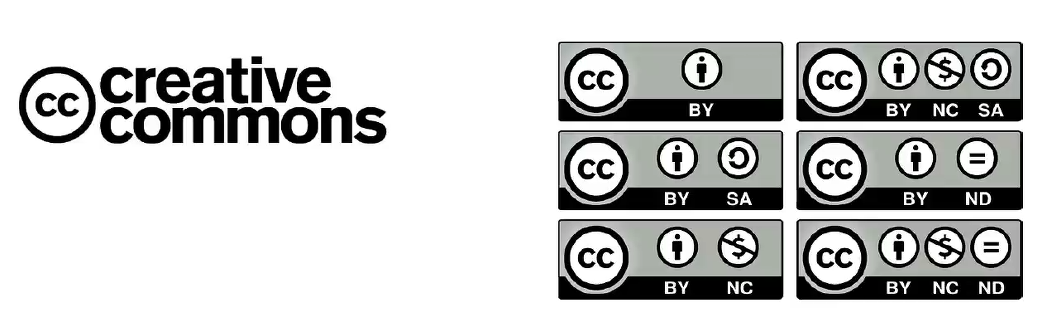
\includegraphics[width=\textwidth]{creative commons 1.png}
    \caption{Licenze Creative Commons}
    \label{creativeCommons1}
\end{figure}

La più vicina al pubblico dominio è la prima in alto a sinistra: è possibile utilizzare un'opera a patto di specificarne l'autore.
\begin{itemize}
    \item BY: è possibile utilizzare un'opera a patto di citarne l'autore (\textit{attribution})
    \item NC: è possibile utilizzare un'opera a patto che non sia per fini commerciali (\textit{non commercial})
    \item ND: \textit{no derivative works}
    \item SA: è permesso distribuire lavori derivati dall'opera solo se con la stessa licenza dell'opera da cui derivano (\textit{share alike})
\end{itemize}

Da queste licenze se ne possono derivare 6 combinazioni, come specificato nell'immagine \ref{creativeCommons1}. 


La SIAE tuttavia non ammette che gli autori possano rilasciare diritti neppure a titolo gratuito, quindi si hanno conflitti con la Creative Commons. 

Creative Commons fu portato in Italia nel 2003. Si tratta di un prodotto molto innovativo dal punto di vista sia tecnologico che giuridico.


Associare una licenza Creative Commons corrisponde ad associare all'opera un \textit{machine-readable digital code} che ne consente il tracciamento; l'utente normalmente vede e dota la sua opera di informazioni grafiche (\textit{commons deed}) che permettono velocemente di capire i possibili utilizzi dell'opera, ma al di sotto si ha una traduzione di questi simboli in un \textit{legal code} che sia supportato dalla legge internazionale (vedi immagine \ref{creativeCommons2}).

\begin{figure}
    \centering
    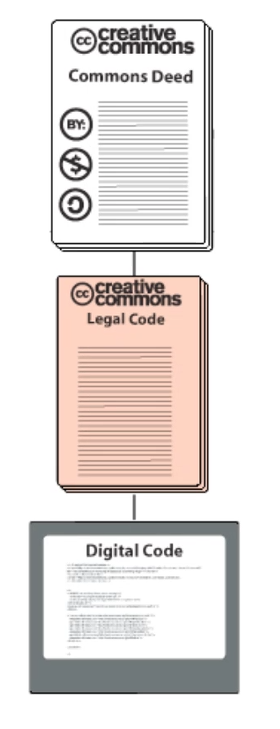
\includegraphics{creative commons 2.png}
    \caption{Creative Commons}
    \label{creativeCommons2}
\end{figure}